\documentclass[11pt, a4paper, twocolumn]{article}
% Packeges
\usepackage{fancyhdr}
\usepackage{graphicx}
\usepackage{listings}
\usepackage{color}

% Fancy header package
\pagestyle{fancy}
\rhead{86411 - Filipe Marques - A097}
\lhead{IArt - Projeto 2}

% Color definitions
\definecolor{dkgreen}{rgb}{0, 0.6, 0}
\definecolor{gray}{rgb}{0.5, 0.5, 0.5}
\definecolor{mauve}{rgb}{0.58, 0, 0.82}

% Listings Settings
\lstset{
	frame=tb,
	language=Python,
	aboveskip=3mm,
	belowskip=3mm,
	showstringspaces=false,
	columns=flexible,
	basicstyle={\small\ttfamily},
	numbers=none,
	numberstyle=\tiny\color{grey},
	keywordstyle=\color{blue},
	commentstyle=\color{dkgreen},
	stringstyle=\color{mauve},
	breaklines=true,
	breakatwhitespace=true,
	tabsize=2
}

% Title
\author{86411 - Filipe dos Santos Oliveira Marques}
\title{Projeto Inteligência Artificial(3º Ano , 1º Semestre 2018/2019)}

\begin{document}
\maketitle
% Parte 1 - Inferência Exata em Redes Bayesianas
\section{Parte 1}
\hspace{10mm}Nesta secção vamos analisar a solução produzida para a primeira parte do segundo projeto da Unidade Curricular de Inteligência Artificial - Inferência Exata em Redes Bayesianas.
\subsection{Análise dos Resultados}
\begin{figure}[h!]
	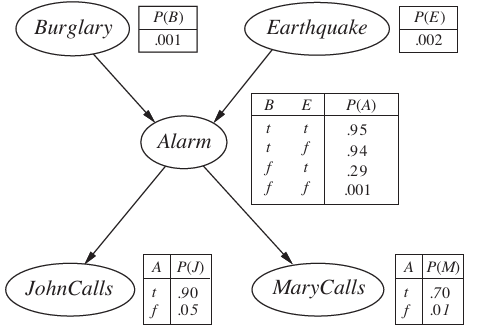
\includegraphics[scale=.45]{images/bn-b.png}
	\caption{Bayesian Network}
	\label{fig:bn1}
\end{figure}
A Figura \ref{fig:bn1} mostra a rede bayesiana utilizada para testar o algoritmos produzidos. %TODO
\subsection{Implementação}
%TODO
\subsubsection{Probabilidade Conjunta}
\hspace{10mm}Para calcular a probabilidade conjunta temos de ter em conta algumas asserções em redes Bayesianas, nomeadamente que:
\begin{itemize}
\item Trata-se de uma rede acíclica; 
\item Cada nó é independente dos seus nós não descentes dado os seus predecessores imediatos(\textit{parents});
\end{itemize}
Sabendo isto, podemos definir a probabilidade conjunta:
\begin{center}
$P(y_{1},...,y_{n}) = \displaystyle\prod_{i=1}^{n}P(y_{i}|Parents(y_{i}))$ 
\end{center}
Onde $Y = \{y_{1},..., y_{n}\}$ representa o conjunto de variáveis na rede Bayesiana.\\
Em Python teriamos:
\begin{lstlisting}
# class BN
def computeJointProb(self, evid):
	p = 1
	for i in range(len(self.prob)):
		p*=self.prob[i].computeProb(evid)[evid[i]]
	return p
\end{lstlisting}
\subsubsection{Probabilidade Posterior}
\hspace{10mm}Para calcular a probabilidade posterior podes usar a probabilidade condicional. Por exemplo, para calcular a probabilidade de haver um \textit{Burglar} sabendo que \textit{JohnCalls} e \textit{MaryCalls} temos:
\begin{center}
$P(B|j=t, m=t)=\displaystyle\frac{P(B,j,m)}{P(j,m)}=\alpha P(B,j,m)$
\end{center}
Para calcular a probabilidade $P(B, j, m)$ temos somar as probabilidades conjuntas para todos os valores de '$e$' e '$a$' onde $j=t$ e $m=t$.\\
Assim:
\begin{center}
$P(B, j, m) = \displaystyle\sum_{e}\sum_{a}P(B, j, m, e, a)$
\end{center}
Tendo conhecimento da rede e das condições de independência podemos reescrever a segunda parte da equação como:
\begin{center}
$\displaystyle\sum_{e}\sum_{a}P(B)P(j|A)P(m|A)P(e)P(A|B,e)$
\end{center}
Agrupando os fatores temos que:
\begin{center}
$P(B)\displaystyle\sum_{e}P(e)\displaystyle\sum_{a}P(A|B, e)P(m|A)P(j|A)$
\end{center}
Esta abordagem de calcular a probabilidade posterior é chamada de enumeração. Para calcular a probabilidade posterior usamos o algoritmo \emph{Enumeration-Ask}[pag.525 - AIMA]
\begin{lstlisting}
def enumerationAsk(X, e, bn):
	Q = [0, 0]
	for xi in [0, 1]:
		e_xi = e.copy()
		Q[xi] = enumerateAll(bn.getVars(), extend(e_xi, X, xi), bn)
	return [Q(0)/sum(Q), Q(1)/sum(Q)]
	
def enumerateAll(vars, e, bn):
	if not vars: return 1
	Y, node = vars[0], bn.getNode(Y)
	rest = vars[1:]
	if isinstance(e[y], int):
		prob = node.computeProb(e)[e[Y]]
		return prob*enumerateAll(rest, e, bn)
	else:
		sumation = 0
		for y in [0, 1]:
			e_y = e.copy()
			prob = node.computeProb(e)[y]
			sumation += prob*enumerateAll(rest, extend(e_y, Y, y), bn)
		return sumation
\end{lstlisting}
\subsection{Complexidade Computacional}
%TODO

% Parte 2 - Aprendizagem por Reforço
\section{Parte 2}
\hspace{10mm}Nesta secção vamos analisar a solução produzida para a segunda parte do segundo projeto da Unidade Curricular de Inteligência Artificial - Aprendizagem por Reforço.
%TODO

\end{document}